\chapter{HASIL DAN PEMBAHASAN}

Bagian ini menyajikan hasil penelitian dalam bentuk data. Selain dengan uraian, data penelitian dapat juga disajikan dalam bentuk ilustrasi (gambar, foto, diagram, grafik, tabel, dll.). Dalam menyajikan tabel atau grafik, hendaknya tabel dan grafik tersebut berupa self explanatory. Artinya, semua keterangan harus ada pada tabel dan grafik tersebut sehingga pembaca dapat memahaminya tanpa harus mengacu kepada teks/naskah.Yang dimaksud dengan pembahasan adalah pemaknaan terhadap data dengan mengaitkannya dengan teori yang sudah dibahas pada bab II. Temuan atau informasi yang diperoleh harus dikaitkan dengan tujuan penelitian (impikasi hasil penelitian).

\section{Gambar}

\begin{figure}[H]
  \centering
  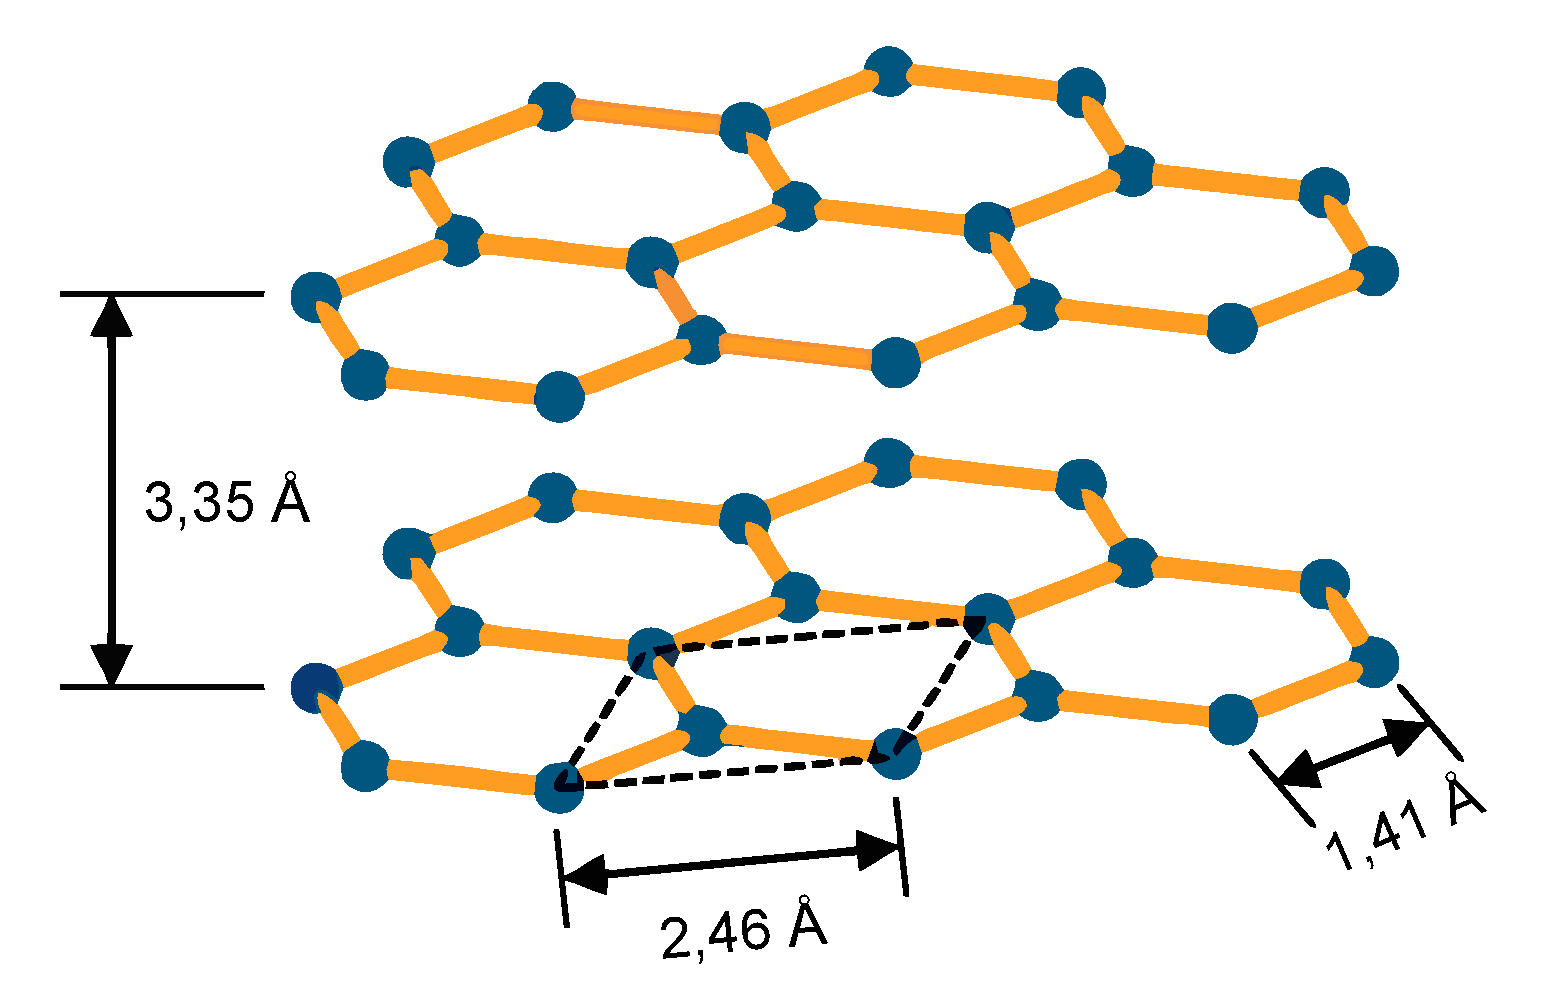
\includegraphics[width=8cm]{Gambar/blg.pdf}
  \caption{Contoh Gambar}
  \label{fig:blg}
\end{figure}

\begin{enumerate}
  \item Gambar dimuat kira-kira di tengah-tengah halaman.
  \item Judulnya ditik di bawah gambar, mengikuti lebar gambar dengan memperhitungkan keseimbangan halaman.
  \item Nomor gambar terdiri atas dua bagian, yaitu:
  \begin{enumerate}[label=(\alph*)]
    \item bagian pertama menunjukkan nomor bab tempat gambar itu dimuat;
    \item bagian kedua menunjukkan nomor urut gambar pada bab itu. Misalnya, Gambar  ~\ref{fig:blg} menunjukkan bahwa gambar itu ada pada Bab IV dan merupakan gambar urutan pertama pada bab itu.
  \end{enumerate}
  \item Kalimat pertama judul gambar ditulis dengan jarak dua ketukan sesudah nomor gambar.
  \item Awal baris kedua judul gambar berada di bawah awal judul gambar (bukan di bawah nomor gambar).
\end{enumerate}

\section{Grafik}
\begin{figure}[H]
  \begin{subfigure}{.5\textwidth}
    \centering
    \includegraphics[width=6.7cm]{Gambar/cv.pdf}
  \end{subfigure}
  \hspace{0.7em}
  \begin{subfigure}{.5\textwidth}
    \centering
    \includegraphics[width=6.7cm]{Gambar/cv_comp.pdf}
  \end{subfigure}
  \caption{Contoh Grafik}
  \label{fig:cv}
  \end{figure}

\begin{enumerate}
  \item Grafik dimuat kira-kira di tengah-tengah halaman.
  \item Judulnya ditik di atas grafik, mengikuti lebar grafik, dengan memperhitungkan keseimbangan halaman.
  \item Nomor grafik terdiri atas dua bagian, yaitu:
  \begin{enumerate}[label=(\alph*)]
    \item bagian pertama menunjukkan nomor bab grafik itu dimuat; 
    \item bagian kedua menunjukkan nomor urut grafik pada bab itu. Misalnya, Gambar  ~\ref{fig:cv} menunjukkan bahwa grafik itu ada pada Bab IV dan merupakan grafik urutan keempat pada bab itu.
  \end{enumerate}
  \item Kalimat pertama judul grafik ditulis dengan jarak dua ketukan sesudah nomor grafik.
  \item Awal baris kedua judul grafik berada di bawah awal judul grafik (bukan di bawah nomor grafik).
\end{enumerate}

\section{Tabel}
\begin{table}[ht!]
  \centering
  \caption{Contoh Tabel}
  \begin{tabular}{|l|l|l|l|l|l|}
  \hline
  \textbf{Sistem} & \textbf{m, n} & \textbf{\begin{tabular}[c]{@{}l@{}}Sudut\\ Puntir (\degree)\end{tabular}} & \textbf{\begin{tabular}[c]{@{}l@{}}Duplikasi\\ ($x \times y \times z$)\end{tabular}} & \textbf{\begin{tabular}[c]{@{}l@{}}Panjang\\ Sistem (\AA)\end{tabular}} & \textbf{\begin{tabular}[c]{@{}l@{}}Jumlah\\ Atom\end{tabular}} \\ \hline
  SLG             & -             & -                                                                  & 1 x 1 x 1                                                                & 35,98                                                                 & 434                                                            \\ \hline
  BLG          & -             & 0                                                                  & 1 x 1 x 1                                                                & 35,98                                                                 & 868                                                            \\ \hline
  tBLG            & 9, 8          & 3,89                                                               & 1 x 1 x 1                                                                & 35,98                                                                 & 868                                                            \\ \hline
  tBLG            & 8, 7          & 4,41                                                               & 1 x 1 x 1                                                                & 31,75                                                                 & 676                                                            \\ \hline
  tBLG            & 5, 3          & 16,43                                                              & 2 x 2 x 1                                                                & 34,20                                                                  & 784                                                            \\ \hline
  \end{tabular}
  \label{tab:str}
  \end{table}

\begin{enumerate}
  \item Tabel dimuat kira–kira di tengah–tengah halaman.
  \item Judulnya ditik di atas tabel, mengikuti lebar tabel, dengan memperhitungkan keseimbangan halaman.
  \item Nomor tabel terdiri atas dua bagian, yaitu:
  \begin{enumerate}[label=(\alph*)]
    \item bagian pertama menunjukkan nomor bab tabel itu dimuat;
    \item bagian kedua menunjukkan nomor urut tabel pada bab itu. Misalnya, Tabel ~\ref{tab:str} menunjukkan bahwa tabel itu berada pada Bab IV dan merupakan tabel urutan pertama pada bab itu.
  \end{enumerate}
  \item Kalimat pertama judul tabel ditulis dengan jarak dua ketukan sesudah nomor tabel.
  \item Awal baris kedua judul tabel berada di bawah awal judul tabel (bukan di bawah nomor tabel).
  \item Ukuran huruf pada isi tabel adalah 10 pt.
  \item Isi tabel ditulis dalam 1 spasi.
\end{enumerate}

\section{Persamaan}

\begin{equation}
  U_{i j}^{\mathrm{LJ}}\left(r_{i j}\right)=4 \epsilon_{i j}\left[\left(\frac{\sigma_{i j}}{r_{i j}}\right)^{12}-\left(\frac{\sigma_{i j}}{r_{i j}}\right)^{6}\right]
\end{equation}

\begin{equation}
  f_{Q}=\frac{C_v(T)}{3Nk_B}=\frac{\displaystyle\int\limits_{0}^{\infty}\frac{u^2e^u}{{(e^u-1)}^2}G(\omega)d\omega}{\displaystyle\int\limits_{0}^{\infty}G(\omega)d\omega}
\end{equation}

\section{Sitasi}
Sitasi dapat dimasukkan seperti ini \cite{moore1998cramming}. Untuk sitasi dengan beberapa sumber, dapat dituliskan juga \cite{wang2020frank,zhang2020molecular}. Atau untuk tiga sumber seperti ini \cite{mcgaughey2019phonon,jiang2015graphene,khan2015equilibrium}.